\documentclass[aspectratio=43,10pt]{beamer}

\usetheme[progressbar=frametitle]{metropolis}
\usepackage{appendixnumberbeamer}
\usepackage{booktabs}
% \usepackage[scale=2]{ccicons}
\usepackage{pgfplots}
\usepgfplotslibrary{dateplot}
\usepackage{xspace}
\usepackage[english,main=brazilian]{babel}
\usepackage[utf8x]{inputenc}
\usepackage[alf]{abntex2cite}
\usepackage{multirow}
\usepackage{ragged2e}
\usepackage{xspace}

\title[]{Uma Implementação Distribuída em Névoa do Algoritmo de Detecção de Novidade em Fluxos de Dados MINAS}
% \subtitle{Seminários de Metodologia Científica}
\author{Luís Henrique Puhl de Souza\\
Orientador: Prof. Dr. Hermes Senger}
\institute{
Universidade Federal de São Carlos \\
Centro de Ciências Exatas e de Tecnologia \\
Departamento de Computação \\
Programa de Pós-Graduação em Ciência da Computação}
% \date{\today}
\date{Fevereiro 2020}
% \titlegraphic{\hfill\includegraphics[height=1.5cm]{logo.pdf}}

\begin{document}

\maketitle

\begin{frame}{Índice}
  \setbeamertemplate{section in toc}[sections numbered]
  \tableofcontents[hideallsubsections]
\end{frame}

\section{Introdução}

\begin{frame} [fragile]{Introdução}
\begin{itemize}

% Contexto Geral
\item Crescimento do número de dispositivos IoT e riscos associados;

% Contexto Específico
\item Detecção de intrusão em redes por novidade

% Proposta
\item Um sistema para detecção de intrusão em Redes IoT implementando em névoa

% hipótese
\item A hipótese do trabalho é que o algoritmo MINAS pode ser distribuído em
nós de nuvem e névoa reduzindo a latência e com pouco comprometimento na
qualidade de detecção.

\end{itemize}
\end{frame}


\section{Fundamentos}
\begin{frame}[fragile]{Fundamentos}
\begin{itemize}
\item Ambientes de computação Distribuída;
\item Plataformas de processamento distribuído de fluxos;
\item Métodos Detecção de Novidade;
\end{itemize}
\end{frame}


\begin{frame}[fragile]{Fundamentos}
\begin{alertblock}{Ambientes de computação Distribuída}
\begin{itemize}
  \item Computação em Nuvem (\emph{Cloud Computing}):
  \\ \textbf{Características:}
  Serviço sob Demanda,
  Amplo acesso à rede,
  Agrupamento de recursos,
  Elasticidade,
  Serviço mensurado;
  \\ \textbf{Implementações:}
    Nuvem privada,
    Nuvem comunitária,
    Nuvem pública,
    Nuvem híbrida
    \cite{NIST2011}.
  
\end{itemize}
\end{alertblock}
\end{frame}

{%
\setbeamertemplate{frame footer}{Terminologia continua incerta entre \emph{fog} e \emph{edge}.}
\begin{frame}[fragile]{Fundamentos}
  \begin{alertblock}{Ambientes de computação Distribuída}
  \begin{itemize}
    
  \item Computação de Borda (\emph{Edge Computing}) \cite{Shi2016}:
  \\ Refere-se a qualquer recurso computacional ou de rede entre os dispositivos
  de borda e centro de dados hospedados em nuvem.
  
  \item Computação em Névoa (\emph{Fog Computing}) \cite{Bonomi2012,dastjerdi2016}:
  \\ \textbf{Características:}
  Mobilidade,
  Heterogeneidade,
  Baixa Latência,
  Distribuição geográfica,
  Alto número de nós,
  Interoperabilidade e federação,
  Uso de fluxo de dados e aplicações em tempo real
  \cite{IEEECommunicationsSociety2018}.
\end{itemize}
\end{alertblock}
\end{frame}
}


\begin{frame}[fragile]{Fundamentos}
\begin{alertblock}{Plataformas de processamento distribuído de fluxos}
  \begin{itemize}
    \item Mineração de Dados e Fluxo de Dados;
    \item Arquiteturas \emph{Lambda} e \emph{Kappa};
    \item \emph{MapReduce} e \emph{Apache Hadoop};
    \item \emph{Apache Spark}, \emph{Resilient Distributed Dataset} e
    \emph{micro-batching} para \emph{Spark Streaming};
    \item \emph{Apache Storm};
    \item \emph{Apache Flink};
  \end{itemize}
\end{alertblock}
\end{frame}

\begin{frame}[fragile]{Fundamentos}
\begin{figure}[ht]
\centering
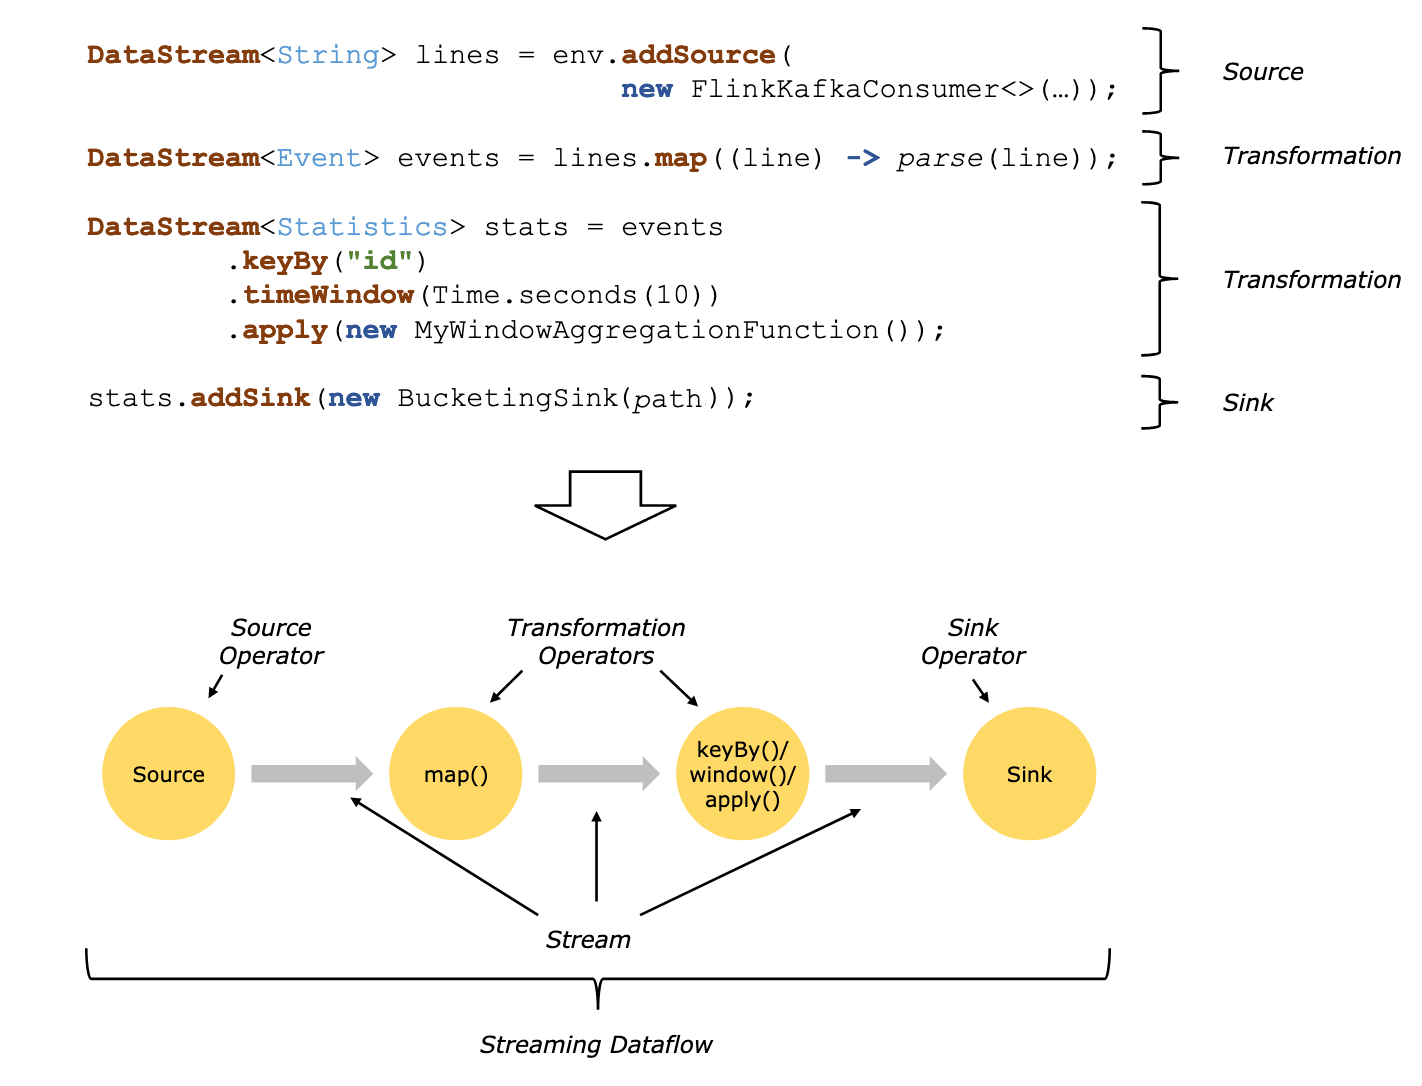
\includegraphics[width=0.85\textwidth]{figuras/dataflow-code-flink.png}
\caption{Exemplo de código e \emph{data flow} do \emph{Apache Flink} \cite{ApacheFlink2020}}
\label{fig:dataflow-flink}
\end{figure}
\end{frame}

\newcommand{\novelty}{\emph{Novelty Detection}\xspace}
\newcommand{\nd}{ND\xspace}
\newcommand{\drift}{\emph{Concept Drift}\xspace}
\newcommand{\evolution}{\emph{Concept Evolution}\xspace}

\begin{frame}[fragile]{Fundamentos}
\begin{alertblock}{Métodos Detecção de Novidade}
  
  \vspace{5mm}
  Métodos Detecção de Novidade (\novelty) lidam com o reconhecimento e
  classificação de exemplos em padrões que diferem de padrões anteriores
  \cite{PERNER2007,Gama2010}.

  Conforme \citeonline{Gama2010}, são características de fluxos de dados contínuos:
  \begin{itemize}
    \item Evolução de conceito (\evolution);
    \item Mudança de conceito (\drift, deriva ou desvio);
    \item Ruído e \emph{outliers};
  \end{itemize}
\end{alertblock}
\end{frame}
\begin{frame}[fragile]{Fundamentos}
\begin{alertblock}{Algoritmo MINAS}
  \vspace{5mm}
  Algoritmo e suas estratégias:
  \begin{itemize}
    \item Modelo de aprendizado \emph{Offline-Online};
    \item Transformação dos dados analisados para o espaço $\mathbb{R}^d$;
    \item Função de classificação baseada em distância euclideana;
    \item Modelo de classificação com \emph{Clusters};
    \item Algoritmo de agrupamento para identificação de padrões;
  \end{itemize}
\end{alertblock}
\end{frame}

\begin{frame}[fragile]{Fundamentos}
\begin{figure}[ht]
\centering
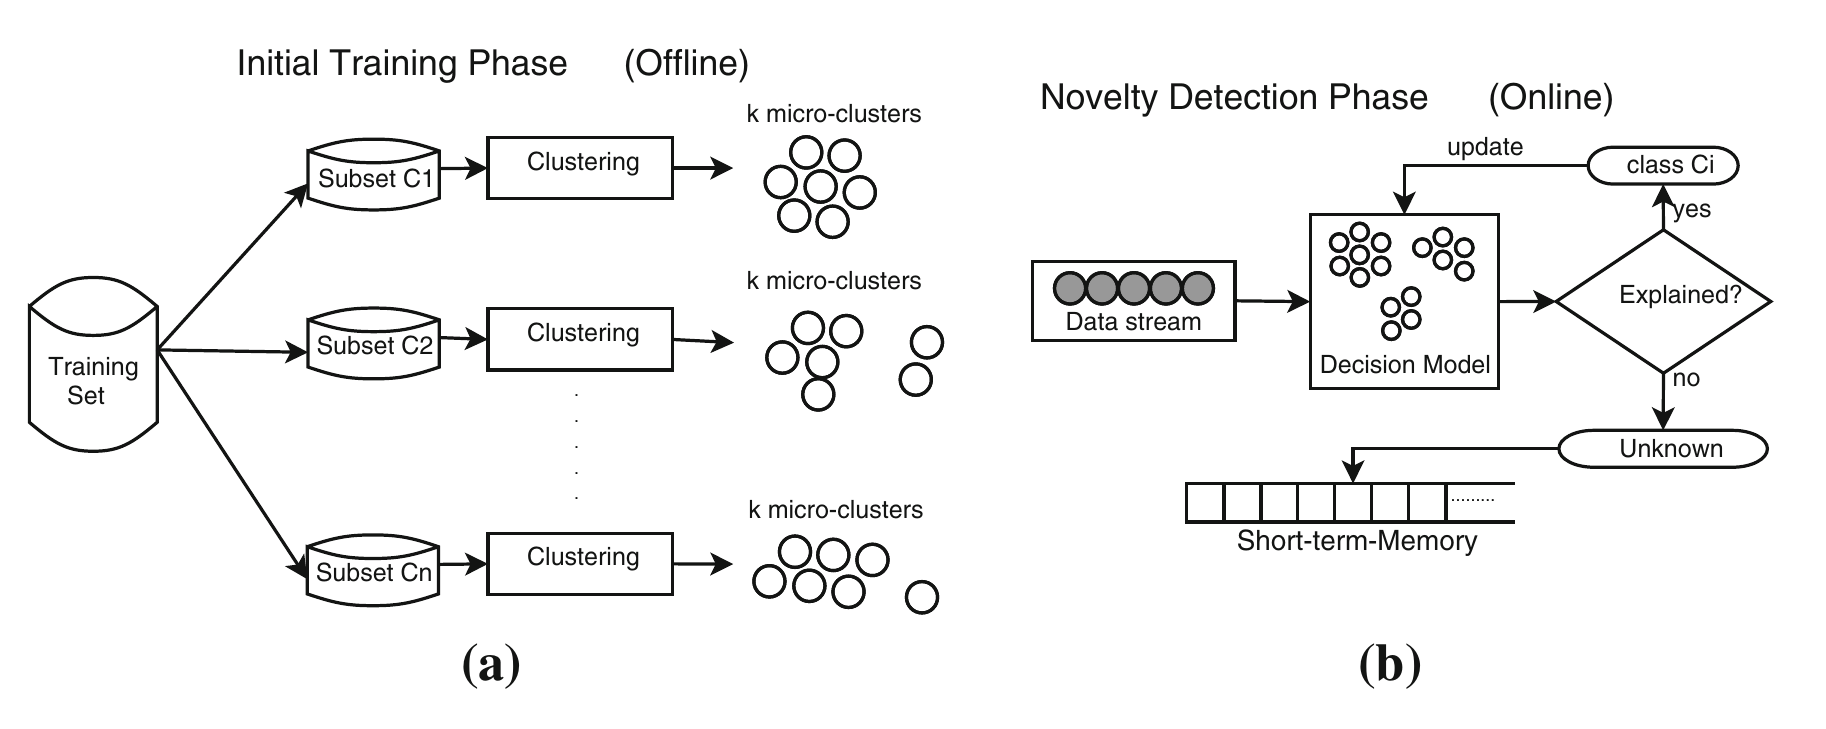
\includegraphics[width=\textwidth]{figuras/FariaMinas2015-fases.png}
\caption{Visão geral do algoritmo MINAS com fases \emph{Offline} (a) e 
\emph{Online} (b) \cite{Faria2016minas}}
\label{fig:minas}
\end{figure}
\end{frame}


\section{Estado da Arte e Trabalhos Relacionados}
\begin{frame}[fragile]{Estado da Arte e Trabalhos Relacionados}
\begin{itemize}
\item Extensões do Algoritmo MINAS;
\item Sistemas de detecção de intrusão em redes;
\end{itemize}
\end{frame}

\begin{frame}[fragile]{Estado da Arte e Trabalhos Relacionados}
\begin{alertblock}{Extensões do Algoritmo MINAS}
  \begin{itemize}
    \item FuzzyND: extensão do algoritmo original para classificação com
    conjunto de etiquetas \emph{fuzzy} \cite{DaSilva2018,DaSilva2018thesis};
    \item MINAS-LC e MINAS-BR: extensão do algoritmo original tratando
    classificação multi-etiquetas \cite{Costa2019,Costa2019thesis};
  \end{itemize}
\end{alertblock}
\end{frame}

\newcommand{\idsiot}{IDSA-IoT\xspace}

\begin{frame}[fragile]{Estado da Arte e Trabalhos Relacionados}
\begin{alertblock}{Sistemas de detecção de intrusão em redes}
  \begin{itemize}
    \item Ferramenta BigFlow \cite{Viegas2019};
    \item Ferramenta CATRACA \cite{Lopez2018};
    \item Arquitetura \idsiot \cite{Cassales2019a};
  \end{itemize}
\end{alertblock}
\end{frame}

\begin{frame}[fragile]{Estado da Arte e Trabalhos Relacionados}
\begin{figure}[ht]
  \centering
  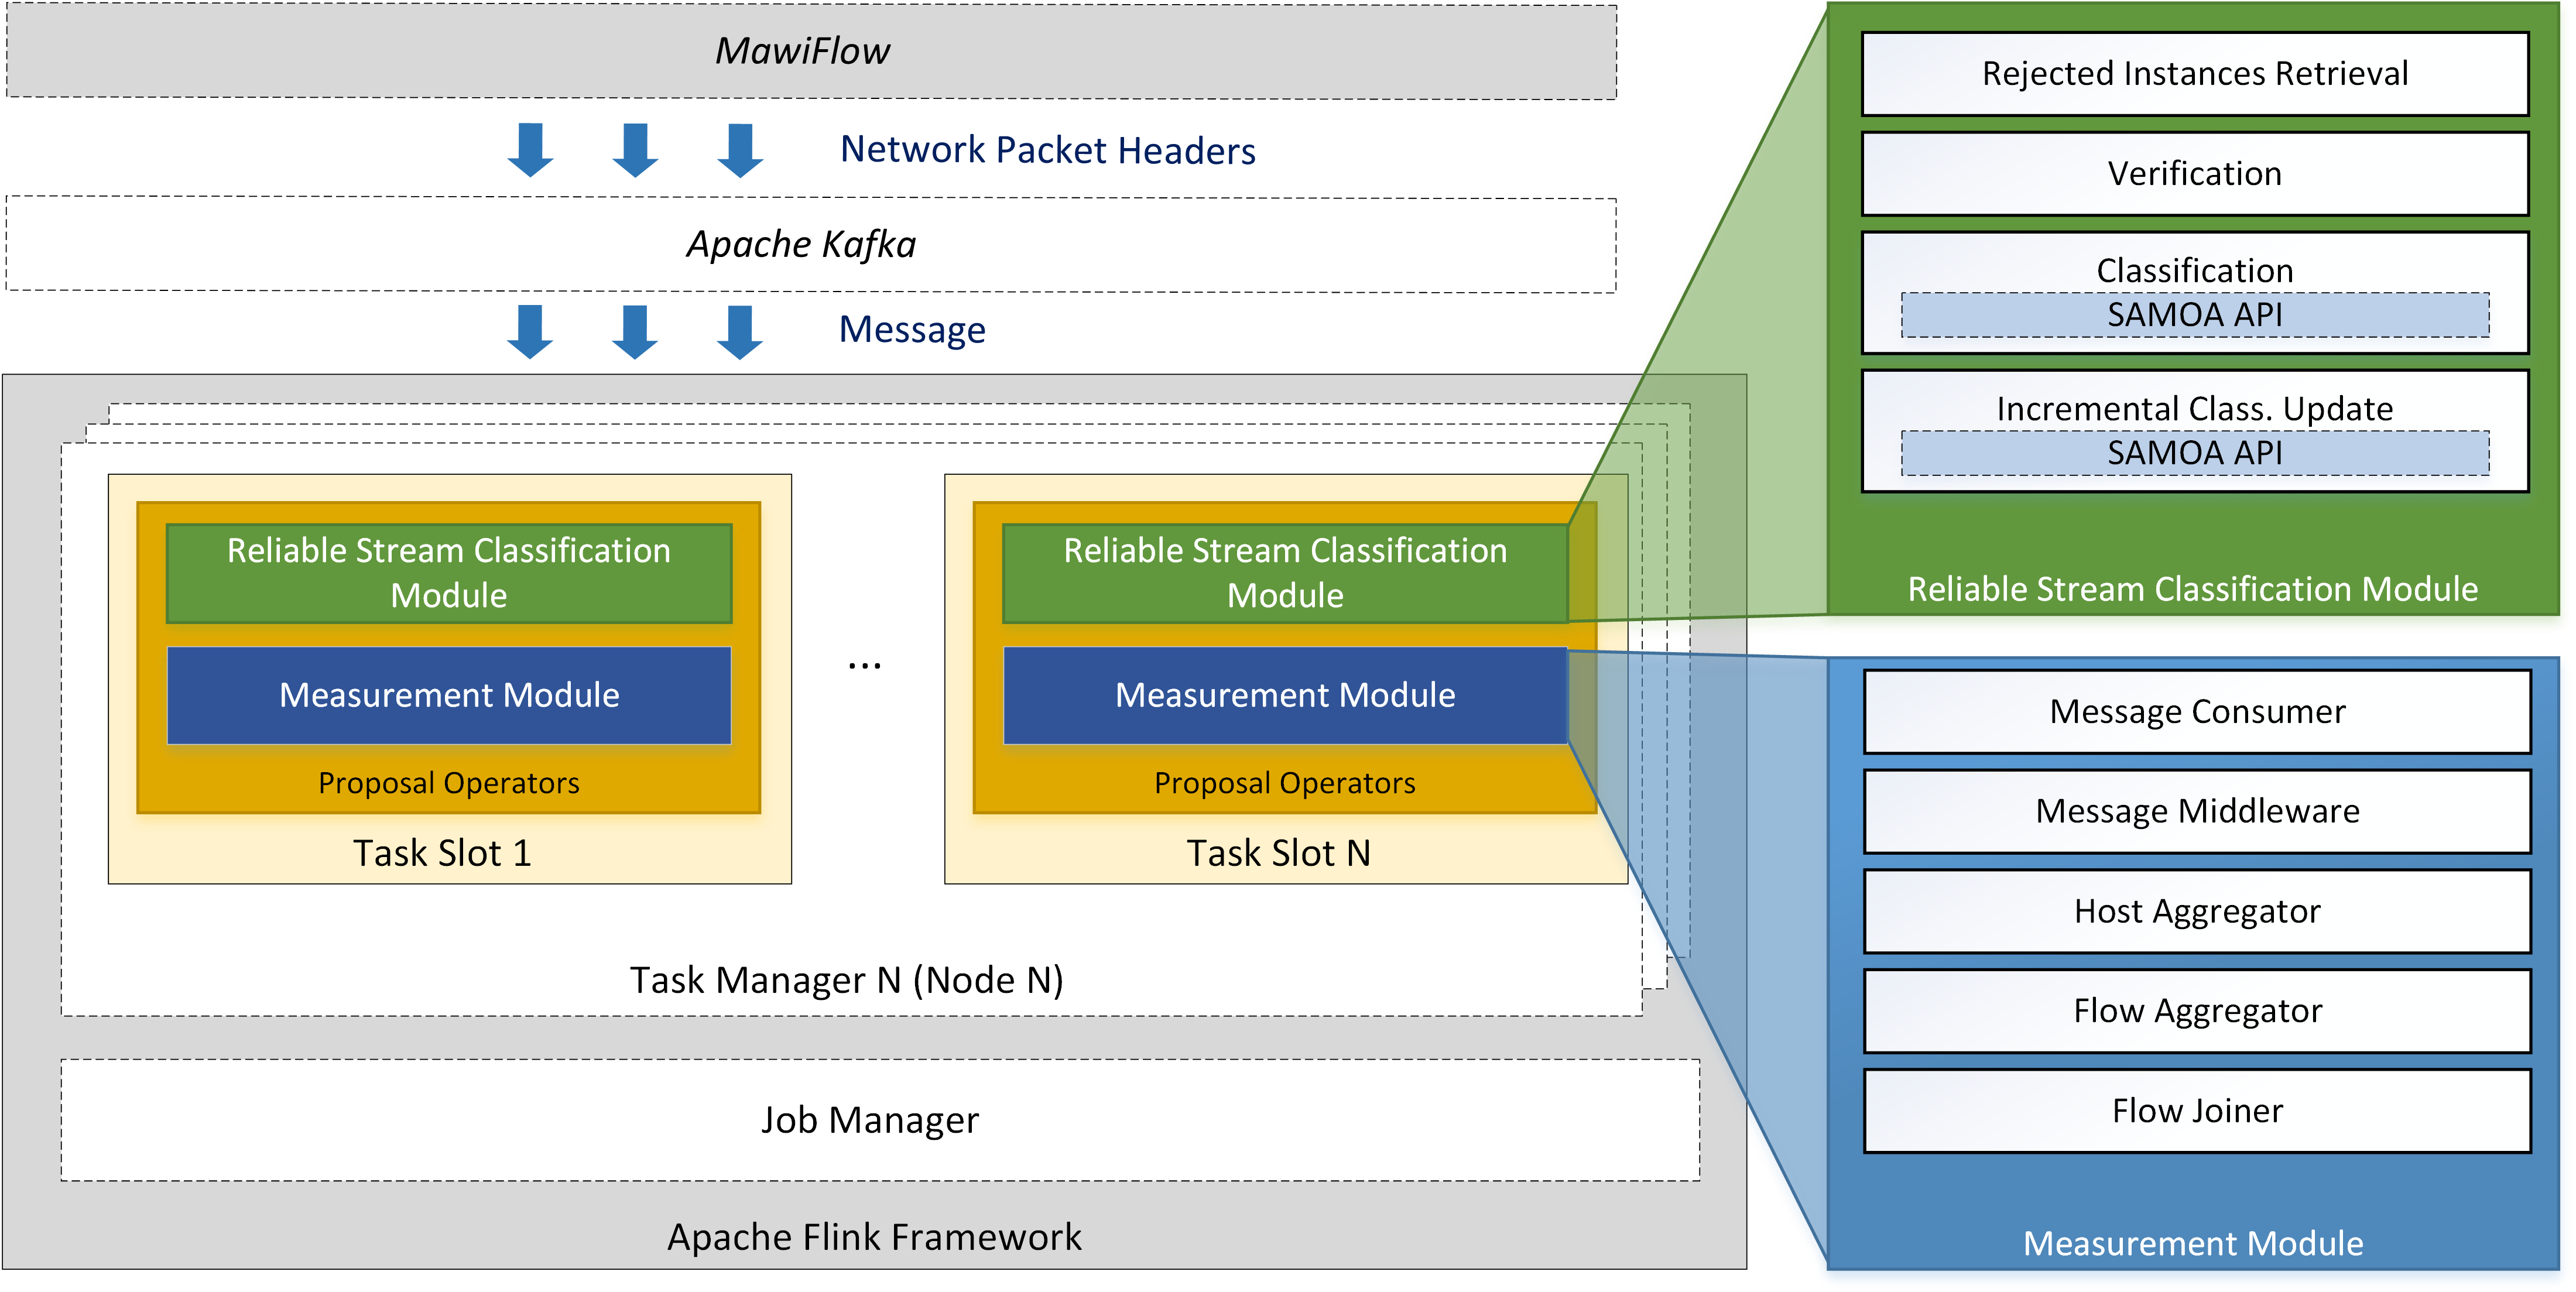
\includegraphics[width=\textwidth]{figuras/bigflow-fig5-bigflow_arch.png}
  \caption{Visão geral da arquitetura e distribuição da ferramenta BigFlow \cite{Viegas2019}.}
  \label{fig:bigflow-arch}
\end{figure}
\end{frame}
\begin{frame}[fragile]{Estado da Arte e Trabalhos Relacionados}
\begin{figure}[ht]
  \centering
  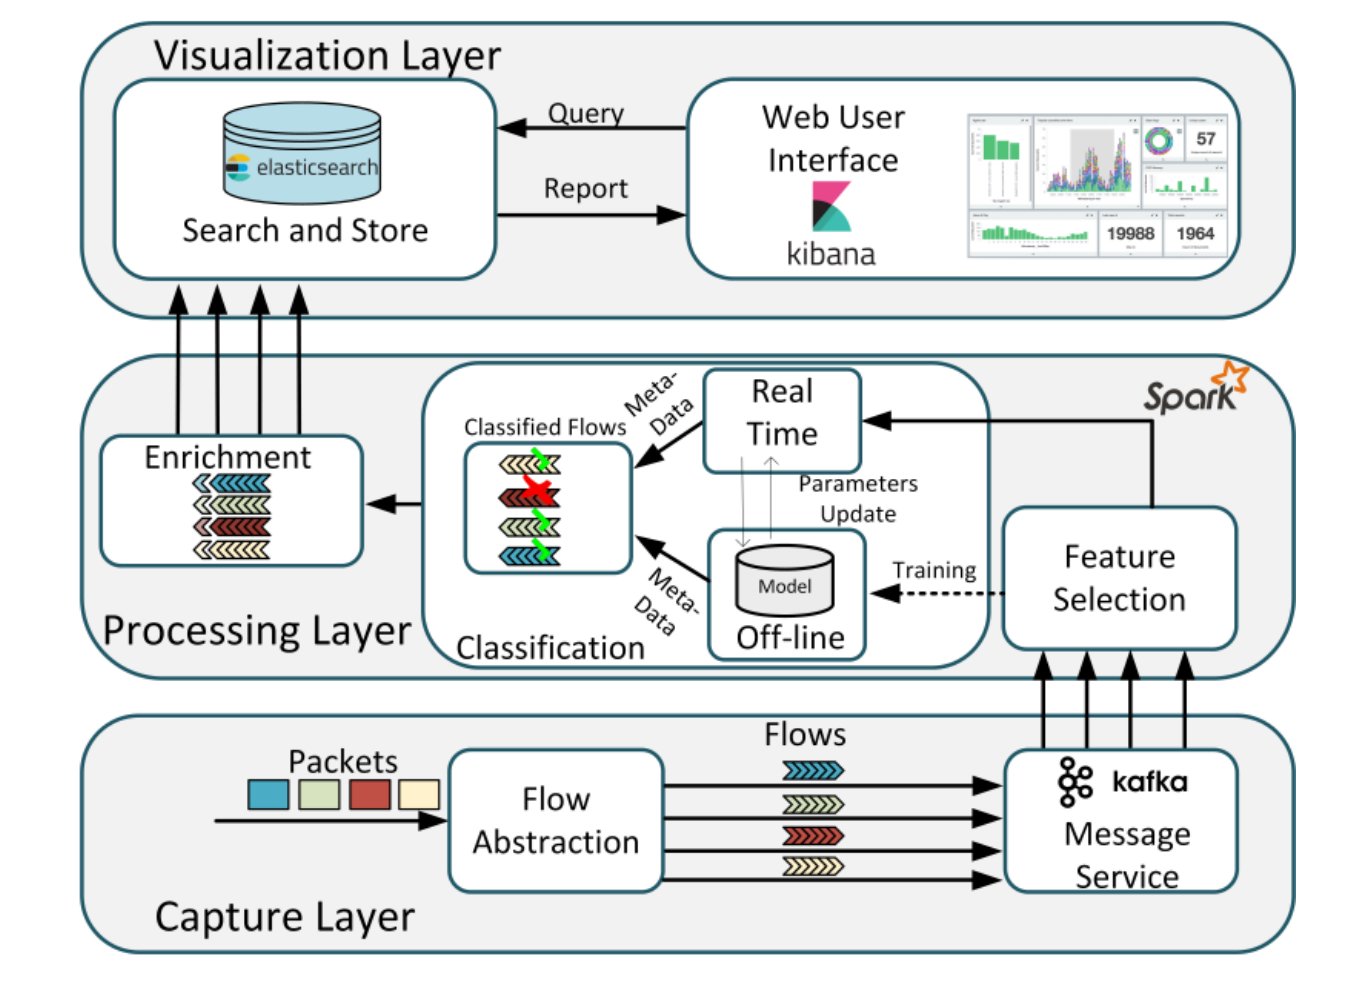
\includegraphics[width=0.8\textwidth]{figuras/catraca-arch.png}
  \caption{Arquitetura em camadas da ferramenta CATRACA \cite{Lopez2018}.}
  \label{fig:catraca}
\end{figure}
\end{frame}
\begin{frame}[fragile]{Estado da Arte e Trabalhos Relacionados}
\begin{figure}[ht]
  \centering
  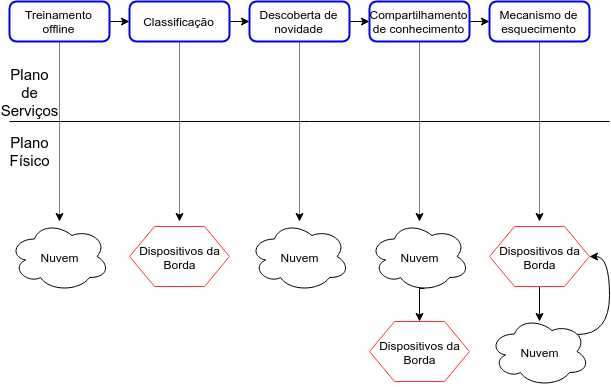
\includegraphics[width=0.8\textwidth]{figuras/idsa-iot-quali-004.png}
  \caption{Distribuição de Serviços da Arquitetura \idsiot.
  Produzida e traduzida por \citeonline{Cassales2019a}.}
  \label{fig:ids-iot}
\end{figure}
\end{frame}

\newcommand{\mfog}{sistema M-FOG\xspace}

\section{Proposta}
\begin{frame}[fragile]{Proposta}
\begin{itemize}
\item Plataforma de processamento distribuído;
\item Arquitetura IDS-IoT;
\item M-FOG e a distribuição do algoritmo MINAS;
\end{itemize}
\end{frame}

\begin{frame}[fragile]{Proposta}
\begin{figure}[h]
  \centering
  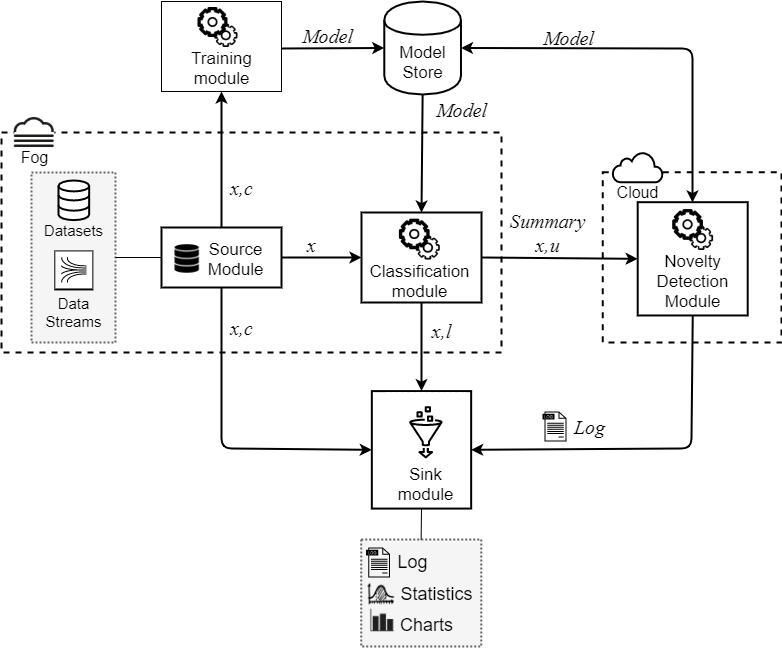
\includegraphics[width=0.8\textwidth]{figuras/mfog.png}
  \caption{Arquitetura e fluxos de dados do \mfog.}
  \label{fig:arch}
\end{figure}
\end{frame}

\section{Resultados Preliminares}
\begin{frame}[fragile]{Resultados Preliminares}
\begin{itemize}
\item Python e Kafka;
\item Flink;
\end{itemize}
\end{frame}

\section{Considerações Finais}
\begin{frame}{Considerações Finais}
Trabalho continua com a finalização da implementação e validação do MFOG com MINAS.
\end{frame}

{\setbeamercolor{palette primary}{fg=black, bg=yellow}\begin{frame}[standout]
  Obrigado!
\end{frame}}

\begin{frame}[allowframebreaks]{Referências}
  \bibliography{99.referencias.bib}
\end{frame}

\appendix

\begin{frame}[fragile]{Recomendações de Leitura}
empty
\end{frame}

\end{document}